
% JuliaCon proceedings template
\documentclass{juliacon}
\setcounter{page}{1}

\begin{document}

% **************GENERATED FILE, DO NOT EDIT**************

\title{My JuliaCon proceeding}

\author[1]{1st author}
\author[1, 2]{2nd author}
\author[2]{3rd author}
\affil[1]{University}
\affil[2]{National Lab}

\keywords{Julia, Optimization, Game theory, Compiler}

\hypersetup{
pdftitle = {My JuliaCon proceeding},
pdfsubject = {JuliaCon 2022 Proceedings},
pdfauthor = {1st author, 2nd author, 3rd author},
pdfkeywords = {Julia, Optimization, Game theory, Compiler},
}



\maketitle

\begin{abstract}

This is a guide for authors who are preparing papers for JuliaCon using the \LaTeX{} document
preparation system and the \verb|juliacon|  class file.

\end{abstract}

\section{Introduction}

The \LaTeX{} document preparation system is a special version of the
\TeX; typesetting program where-in a collection of \TeX; commands
are added to \LaTeX{} to simplify typesetting. Importantly, it allows
the author to concentrate on the logical structure of the document
rather than its visual layout.\vskip 6pt
Moreover, \LaTeX{} provides a consistent and comprehensive document
preparation interface. There are simple-to-use commands for
generating a table of contents, lists of figures and/or tables, and indexes.
\LaTeX{} can automatically number list entries, equations, figures,
tables, and footnotes, as well as articles, sections, and subsections.
Using this numbering system, bibliographic citations, page
references, and cross references to any other numbered entity (e.g.
article, section, equation, figure, list entry, etc.) become quite simple
and straightforward. The use of \LaTeX{} document classes allows
a simple change of class to transform the appearance of your document.\vskip 6pt
\LaTeX{} is a powerful tool for managing long and complex documents.
In particular, partial processing enables long documents to
be produced article by article without losing sequential information.
The use of document classes allows a simple change of style
(or style option) to transform the appearance of your document.



\section{The JuliaCon Article Class}
\label{sec:documentclass}
%
The juliacon class file preserves the standard LATEX{} interface such
that any document that can be produced using the standard LATEX{}
article class can also be produced with the class file.\vskip 6pt
It is likely that the make up will change after file submission. For
this reason, we ask you to ignore details such as slightly long lines,
page stretching, or figures falling out of synchronization, as these
details can be dealt with at a later stage.\vskip 6pt
Use should be made of symbolic references (\verb|\ref| ) in order to
protect against late changes of order, etc.

\section{USING THE JuliaCon Article CLASS FILE}

If the file \verb|juliacon.cls|  is not already in the appropriate system directory
for \LaTeX{} files, either arrange for it to be put there or copy
it to your working directory. The \verb|juliacon|  document class is implemented
as a complete class, not a document style option. In order to
use the \verb|juliacon  document class, replace \verb|article|  by \verb|juliacon|  in the
\verb|\documentclass|  command at the beginning of your document:
\vskip 6pt
\begin{centering}
    \verb|\documentclass{article}|  \end{centering}
\vskip 6pt
replace by
\vskip 6pt
 \verb|\documentclass{juliacon}|  \vskip 6pt
In general, the following standard document \verb|style|  options should
{ \itshape not} be used with the {\footnotesize \itshape article} class file:
\begin{enumerate}
\item[(1)] \verb|10pt|,  \verb|11pt|,  \verb|12pt|   ? unavailable;
\item[(2)] \verb|twoside|  (no associated style file) ? \verb|twoside|  is the default;
\item[(3)] \verb|fleqn|, \verb|leqno|, \verb|titlepage| ? should not be used;
\end{enumerate}

\section{Additional Document Style Options}
\label{sec:additional_doc}
%
The following additional style option is available with the \verb|juliacon|  class file:
\vskip 6pt
Please place any additional command definitions at the very start of
the \LaTeX{} file, before the \verb|\begin{document}|. For example, user-defined
\verb|\def|  and \verb|\newcommand|   commands that define macros for
technical expressions should be placed here. Other author-defined
macros should be kept to a minimum.
\vskip 6pt
Commands that differ from the standard \LaTeX{} interface, or that
are provided in addition to the standard interface, are explained in
this guide. This guide is not a substitute for the \LaTeX{} manual itself.
Authors planning to submit their papers in \LaTeX{} are advised to use
\verb|juliacon.cls|  as early as possible in the creation of their files.

%
%
%
%
\begin{table*}[t]
\tabcolsep22pt
\tbl{If necessary, the tables can be extended both columns.}{
\begin{tabular}{|l|l|c|c|}\hline
Label & \multicolumn{1}{c|}{Description}
& Number of Users &
Number of Queries\\\hline
Test 1 & Training Data &
\smash{\raise-7pt\hbox{70}} & 104\\
\cline{1-2}\cline{4-4}
Test 2 & Testing Data I & & 105\\\hline
Test 3 & Testing Data II & 30 & 119\\\hline
& Total & 100 & 328\\\hline
\end{tabular}}
\label{tab:symbols}
\begin{tabnote}
This is an example of table footnote.
\end{tabnote}
\end{table*}
% \begin{figure*}[t]
% \centerline{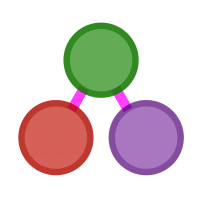
\includegraphics[width=11cm]{juliagraphs.png}}
% \caption{If necessary, the images can be extended both columns.}
%   \label{fig:sample_image}
% \end{figure*}

\section{Additional features}
\label{sec:additional_faci}
In addition to all the standard \LaTeX{} design elements, the \verb|juliacon|  class file includes the following features:
In general, once you have used the additional \verb|juliacon.cls| facilities
in your document, do not process it with a standard \LaTeX{} class
file.

\subsection{Titles, Author's Name, and Affiliation}
\label{subsub:title_auth}
The title of the article, author's name, and affiliation are used at the
beginning of the article (for the main title). These can be produced
using the following code:

\begin{verbatim}
\title{ This is an example of article title} }
\author{
   \large 1st Author \\[-3pt]
   \normalsize 1st author's affiliation  \\[-3pt]
    \normalsize 1st line of address \\[-3pt]
    \normalsize 2nd line of address \\[-3pt]
    \normalsize	1st author's email address \\[-3pt]
  \and
   \large 2nd Author \\[-3pt]
   \normalsize 2nd author's affiliation  \\[-3pt]
    \normalsize 1st line of address \\[-3pt]
    \normalsize 2nd line of address \\[-3pt]
    \normalsize	2nd author's email address \\[-3pt]
\and
   \large 3rd Author \\[-3pt]
   \normalsize 3rd author's affiliation  \\[-3pt]
    \normalsize 1st line of address \\[-3pt]
    \normalsize 2nd line of address \\[-3pt]
    \normalsize	3rd author's email address \\[-3pt]
}
\maketitle
\end{verbatim}

\subsection{Writing Julia code}

A special environment is already defined for Julia code,
built on top of \textit{listings} and \textit{jlcode}.

\begin{verbatim}
\begin{lstlisting}[
    language = Julia, 
    numbers=left, 
    label={lst:exmplg}, 
    caption={Example Code Block.}
]
using Plots

x = -3.0:0.01:3.0
y = rand(length(x))
plot(x, y)
\end{lstlisting}
\end{verbatim}
\begin{lstlisting}[
    language = Julia, 
    numbers=left, 
    label={lst:exmplg}, 
    caption={Example Code Block.}
]
using Plots

x = -3.0:0.01:3.0
y = rand(length(x))
plot(x, y)
\end{lstlisting}


\subsection{Abstracts, Key words, term etc...}
\label{subsub:abs_key_etc}

At the beginning of your article, the title should be generated
in the usual way using the \verb|\maketitle|  command. For genaral tem and keywords use
\verb|\terms|,
\verb|\keywords|  commands respectively. The abstract should be enclosed
within an abstract environment, All these environment
can be produced using the following code:
\begin{verbatim}
\terms{Experimentation, Human Factors}

\keywords{Face animation, image-based modelling...}

\begin{abstract}
In this paper, we propose a new method for the
systematic determination of the model's base of
time varying delay system. This method based on
the construction of the classification data related
to the considered system. The number, the orders,
the time delay and the parameters of the local
models are generated automatically without any
knowledge about the full operating range of the
process. The parametric identification of the local
models is realized by a new recursive algorithm for
on line identification of systems with unknown time
delay. The proposed algorithm allows simultaneous
estimation of time delay and parameters of
discrete-time systems. The effectiveness of
the new method has been illustrated through
simulation.
\end{abstract}

\end{verbatim}

\section{Some guidelines}
\label{sec:some_guide}
The following notes may help you achieve the best effects with the
\verb|juliacon|  class file.

\subsection{Sections}
\label{subsub:sections}
\LaTeXe{}  provides four levels of section headings and they are all
defined in the \verb|juliacon|  class file:
\begin{itemize}
\item \verb|\section|
\item \verb|\subsection|
\item \verb|\subsubsection|
\item \verb|\paragraph|
\end{itemize}
Section headings are automatically converted to allcaps style.
\subsection{Lists}
\label{sec:lists}
%
The \verb|juliacon|   class file provides unnumbered lists using the
\verb|unnumlist|  environment for example,

\begin{unnumlist}
\item First unnumbered item which has no label and is indented from the
left margin.
\item Second unnumbered item.
\item Third unnumbered item.
\end{unnumlist}
The unnumbered list which has no label and is indented from the
left margin. was produced by:
\begin{verbatim}
\begin{unnumlist}
\item First unnumbered item...
\item Second unnumbered item...
\item Third unnumbered item...
\end{unnumlist}
\end{verbatim}

The \verb|juliacon|  class file also provides hyphen list using the
\verb|itemize|  environment for example,
\begin{itemize}
\item First unnumbered bulleted item which has no label and is indented
from the left margin.
\item Second unnumbered bulleted item.
\item Third unnumbered bulleted item which has no label and is indented
from the left margin.
\end{itemize}
was produced by:
\begin{verbatim}
\begin{itemize}
\item First item...
\item Second item...
\item Third item...
\end{itemize}
\end{verbatim}

Numbered list is also provided in acmtog class file using the
enumerate environment for example,
\begin{enumerate}
\item The attenuated and diluted stellar radiation.
\item Scattered radiation, and
\item Reradiation from other grains.
\end{enumerate}

was produced by:
\begin{verbatim}
\begin{enumerate}
\item The attenuated...
\item Scattered radiation, and...
\item Reradiation from other grains...
\end{enumerate}
\end{verbatim}
\subsection{Illustrations (or figures)}
\label{subsub:sec_Illus}
The \verb|juliacon|  class file will cope with most of the positioning of
your illustrations and you should not normally use the optional positional
qualifiers on the \verb|figure|  environment that would override
these decisions.
\vskip 6pt

%
\begin{figure}[t]
\centerline{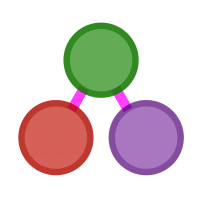
\includegraphics[width=4cm]{juliagraphs.png}}
\caption{This is example of the image in a column.}
	\label{fig:sample_figure}
\end{figure}

The figure \ref{fig:sample_figure} is taken from the JuliaGraphs
organization \footnote{https://github.com/JuliaGraphs}.

Figure captions should be \emph{below} the figure itself, therefore the
\verb|\caption|  command should appear after the figure or space left for
an illustration. For example, Figure 1 is produced using the following
commands:

\begin{verbatim}
\begin{figure}
\centerline{\includegraphics[width=20pc]{Graphics.eps}}
\caption{An example of the testing process for a
binary tree. The globa null hypothesis is tested
first at level $\alpha$ (a), and the level of
individual variables is reached last (d). Note
that individual hypotheses can be tested at
level $\alpha/4$ and not $\alpha/8$ as one might
expect at first.}
\label{sample-figure_2}
\end{figure}
\end{verbatim}
Figures can be resized using first and second argument of
\verb|\includegraphics|   command. First argument is used for modifying
figure height and the second argument is used for modifying
figure width respectively.
\vskip 6pt
Cross-referencing of figures, tables, and numbered, displayed
equations using the \verb|\label|  and \verb|\ref|   commands is encouraged.
For example, in referencing Figure 1 above, we used
\verb|Figure~\ref{sample-figure}|

 \subsection{Tables}
\label{subsub:sec_Tab}
The \verb|juliacon|   class file will cope with most of the positioning of
your tables and you should not normally use the optional positional qualifiers on the table environment which would override these
decisions. Table captions should be at the top.
\begin{verbatim}
\begin{table}
\tbl{Tuning Set and Testing Set}{
\begin{tabular}{|l|l|c|c|}\hline
Label & \multicolumn{1}{c|}{Description}
& Number of Users &
Number of Queries\\\hline
Train70 & Training Data &
\smash{\raise-7pt\hbox{70}} & 104\\
\cline{1-2}\cline{4-4}
Test70 & Testing Data I & & 105\\\hline
Test30 & Testing Data II & 30 & 119\\\hline
& Total & 100 & 328\\\hline
\end{tabular}}
\end{table}
\end{verbatim}

\begin{table}
\tbl{Tuning Set and Testing Set}{
\begin{tabular}{|l|l|c|c|}\hline
Label & \multicolumn{1}{c|}{Description}
& Number of Users &
Number of Queries\\\hline
Test 1 & Training Data &
\smash{\raise-7pt\hbox{70}} & 104\\
\cline{1-2}\cline{4-4}
Test 2 & Testing Data I & & 105\\\hline
Test 3 & Testing Data II & 30 & 119\\\hline
& Total & 100 & 328\\\hline
\end{tabular}}
\end{table}
\subsection{Landscaping Pages}
\label{subsub:landscaping_pages}
If a table is too wide to fit the standard measure, it may be turned,
with its caption, to 90 degrees. Landscape tables cannot be produced
directly using the \verb|juliacon|   class file because \TeX{} itself cannot
turn the page, and not all device drivers provide such a facility.
The following procedure can be used to produce such pages.
\vskip 6pt
Use the package \verb|rotating|   in your document and change the coding
from
\begin{verbatim}
\begin{table}...\end{table}
to
\begin{sidewaystable}...\end{sidewaystable}
and for figures
\begin{figure}...\end{figure}
to
\begin{sidewaysfigure}...\end{sidewaysfigure}
\end{verbatim}

environments in your document to turn your table on the appropriate
page of your document. For instance, the following code prints
a page with the running head, a message half way down and the
table number towards the bottom.
\begin{verbatim}
\begin{sidewaystable}
\tbl{Landscape table caption to go here.}{...}
\label{landtab}
\end{sidewaystable}
\end{verbatim}

\subsection{Double Column Figure and Tables}
\label{subsub:double_fig_tab}
For generating the output of figures and tables in double column
we can use the following coding:

\begin{enumerate}
\item For Figures:
\begin{verbatim}
\begin{figure*}...\end{figure*}
\end{verbatim}
\item For landscape figures:
\begin{verbatim}
\begin{sidewaysfigure*}...\end{sidewaysfigure*}
\end{verbatim}
\item For Tables:
\begin{verbatim}
\begin{table*}...\end{table*}
\end{verbatim}
\item For landscape tables:
\begin{verbatim}
\begin{sidewaystable*}...\end{sidewaystable*}
\end{verbatim}
\end{enumerate}

\subsection{Typesetting Mathematics}
\label{subsub:type_math}
The \verb|juliacon| class file will set displayed mathematics with center to
the column width, provided that you use the \LaTeXe{} standard of
open and closed square brackets as delimiters.
The equation
\[
\sum_{i=1}^p \lambda_i = (S)
\]

was typeset using the acmtog class file with the commands

\begin{verbatim}
\[
\sum_{i=1}^p \lambda_i = (S)
\]
\end{verbatim}

For display equations, cross-referencing is encouraged. For example,
\begin{verbatim}
\begin{equation}
(n-1)^{-1} \sum^n_{i=1} (X_i - \overline{X})^2.
\label{eq:samplevar}
\end{equation}
Equation~(\ref{eq:samplevar}) gives the formula for
sample variance.
\end{verbatim}
The following output is generated with the above coding:
\begin{equation}
(n-1)^{-1} \sum^n_{i=1} (X_i - \overline{X})^2.
\label{eq:samplevar}
\end{equation}
Equation~(\ref{eq:samplevar}) gives the formula for
sample variance.


\subsection{Enunciations}
\label{subsub:enunciation}
The \verb|juliacon|   class file generates the enunciations with the help of
the following commands:
\begin{verbatim}
\begin{theorem}...\end{theorem}
\begin{strategy}...\end{strategy}
\begin{property}...\end{property}
\begin{proposition}...\end{proposition}
\begin{lemma}...\end{lemma}
\begin{example}...\end{example}
\begin{proof}...\end{proof}
\begin{definition}...\end{definition}
\begin{algorithm}...\end{algorithm}
\begin{remark}...\end{remark}
\end{verbatim}
The above-mentioned coding can also include optional arguments
such as
\begin{verbatim}
\begin{theorem}[...]. Example for theorem:
\begin{theorem}[Generalized Poincare Conjecture]
Four score and seven ... created equal.
\end{theorem}
\end{verbatim}

\begin{theorem}[Generalized Poincare Conjecture]
Four score and seven years ago our fathers brought forth,
upon this continent, a new nation, conceived in Liberty,
 and dedicated to the proposition that all men are
created equal.
\end{theorem}


\subsection{Extract}
\label{subsub:extract}
Extract environment should be coded within
\begin{verbatim}
\begin{extract}..\end{extract}
\end{verbatim}

\subsection{Balancing column at last page}
\label{subsub:Balance}
For balancing the both column length at last page use :
\begin{verbatim}
\vadjust{\vfill\pagebreak}
\end{verbatim}

%\vadjust{\vfill\pagebreak}

at appropriate place in your \TeX{} file or in bibliography file.

\section{Handling references}
\label{subsub:references}
References are most easily (and correctly) generated using the
BIBTEX, which is easily invoked via
\begin{verbatim}
\bibliographystyle{juliacon}
\bibliography{ref}
\end{verbatim}
When submitting the document source (.tex) file to external
parties, the ref.bib file should be sent with it.
\cite{bezanson2017julia}

% **************GENERATED FILE, DO NOT EDIT**************

\bibliographystyle{juliacon}
\bibliography{ref.bib}


\end{document}

% Inspired by the International Journal of Computer Applications template
